\documentclass[a4paper]{article}

\usepackage[utf8]{inputenc}
\usepackage[portuges]{babel}
\usepackage{amsmath}
\usepackage{graphicx}
\usepackage{a4wide}
\usepackage[pdftex]{hyperref}
\usepackage{float}
\usepackage{indentfirst}
\usepackage{subcaption}
\usepackage{bm}
\usepackage{amssymb}


\usepackage{listings}

\usepackage{algorithm}
\usepackage[noend]{algpseudocode}

\begin{document}

\title{Trabalho Prático\\ Agentes Inteligentes\\Grupo 3}
\author{Bruno Martins (a80410) \and Catarina Machado (a81047) \and Filipe Monteiro (a80229)}
\date{\today}

\begin{titlepage}

  %título
  \thispagestyle{empty}
  \begin{center}
  \begin{minipage}{0.75\linewidth}
      \centering
  %engenharia logo
      
\includegraphics[width=0.4\textwidth]{eng.png}\par\vspace{1cm}
      \vspace{1.5cm}
  %titulos
      \href{https://www.uminho.pt/PT}{\scshape\LARGE Universidade do Minho} \par
      \vspace{1cm}
      \href{https://www.di.uminho.pt/}{\scshape\Large Departamento de Informática} \par
      \vspace{1.5cm}

\maketitle
\end{minipage}
\end{center}

\clearpage

\end{titlepage}

\tableofcontents

\pagebreak

\section{Introdução}

Os Sistemas Multiagentes são uma subárea da Inteligência Artificial Distribuída e concentram-se no estudo de agentes autónomos no universo multiagente. Neste sistema, três ou mais agentes interagem entre si e trabalham cooperativamente ou competitivamente para atingir um objetivo. Paralelismo, escalabilidade e a possibilidade de divisão em problemas menores são as principais características destes sistemas.

O objetivo do sistema multiagente do presente trabalho prático é monitorizar e resolver catástrofes naturais, através da aplicação de vários sensores virtuais de captura de localização GPS, representados por agentes.

O cenário do nosso problema consiste num simulador de combate a incêndios florestais. Neste simulador, existirão Agentes Participativos, que são os veículos autónomos e inteligentes (voadores e terrestres), mais especificamente aeronaves, drones e camiões de bombeiros. Para além disso, existirá um Agente Central, o quartel de bombeiros, responsável pela monitorização, coordenação e distribuição de tarefas entre os agentes participativos.

Desta forma, começaremos por apresentar um estado da arte sobre os agentes e a sua aplicação em domínios concretos, abordando as diferentes propriedades, e, em seguida, explicamos como pensamos, concebemos e modelamos uma arquitetura distribuída baseada em agentes para o dado problema. Para isso, começamos por expor a Contextualização geral da nossa solução, seguido da sua Arquitetura geral, e, posteriormente, o respetivo Protocolo de Comunicação. Por fim, abordamos o Processamento Interno dos Agentes. Em cada um dos três últimos tópicos mencionados foram aplicadas metodologias \textit{Agent UML} para formalizar os protocolos de interação entre agentes.

\section{Estado de Arte}
\subsection{Descrição do Problema}
O nosso sistema multiagente consiste num simulador de combate a incêndios florestais. Neste sistema, existem três diferentes tipos de agentes: os agentes participativos, que são os veículos autónomos e inteligentes (voadores e terrestres), tais como aeronaves, drones e camiões de bombeiros; o agente central, ou seja, o quartel, que é responsável por coordenar e distribuir tarefas entre os agentes participativos. Estas decisões são influenciadas por um conjunto de fatores existentes no meio, nomeadamente as localizações de locais de abastecimento disponíveis de água e combustível. Por fim, existe um agente secundário, o ateador de fogos, que gerará incêndios em momentos/posições aleatórias.

O objetivo do sistema é monitorizar e resolver estas catástrofes naturais, de forma a que todos os fogos sejam apagados o mais rapidamente possível, colmatando assim num ambiente livre de chamas.

\subsection{Revisão da Literatura}
O sistema que estamos a desenvolver basear-se-á na existência de uma organização de agentes que, cooperando entre si irão resolver um problema. Neste caso, estes agentes irão “tratar” o problema por completo, mas, na sua essência, seria para ajudar na alocação de recursos, otimização de rotas, na própria gestão do meio. 

Atualmente, já vários estudos foram feitos na área, onde se procura criar uma plataforma que consiga gerir, eficientemente, uma força de ajuda no caso de um desastre natural. Isto, porque o ser Humano é limitado, podendo dar resposta, da melhor forma, a um número pequeno de ocorrências comparativamente a uma máquina. Também o fazem com falta de informação do panorama geral, às vezes provocando decisões não tão acertadas. Com uma máquina, esta sabendo o estado por completo dos recursos, das zonas de perigo, entre outros fatores, pode tomar as decisões mais lógicas possíveis, indicando simplesmente aos respetivos meios de combate o que é necessário.

Em 2010, um estudo foi feito na criação de um sistema de multiagentes capaz de auxiliar as equipas de resgate no caso de um desastre natural, no Paquistão, depois de um enorme tremor de terra, em 2006, ter tido um efeito devastador, onde as equipas de resgate se encontraram “presas” pela gravidade da situação. Esta plataforma, chamada de \textbf{FMSIND}\cite{fmsind} (\textit{A Framework of Multi-Agent Systems Interaction during Natural Disaster}), consistia numa grande divisão de tarefas por variadíssimos agentes, onde no final, um último agente iria fazer a comunicação ao respetivo serviço de ajuda (bombeiros, polícias, médicos, entre outros). Arquiteturalmente consiste no seguinte:

Um agente detentor de sensores (\textbf{Sensor Agent}) fica à escuta de um desastre. Após estímulo, notifica um sistema de decisão do tipo de desastre (\textbf{DSS}) que irá avaliar a situação e enviar o que necessita para resolução do problema de volta para o agente sensorial. Este por sua vez irá enviar ao agente supervisor (\textbf{Supervisor Agent}) o que necessita e o agente supervisor irá distribuir a gestão dos diferentes tipos de recursos pelos diferentes agentes responsáveis por cada área (\textbf{On-Site Agents}). Cada um destes, depois de comunicar com a base de dados sobre os recursos disponíveis, irá comunicar com o seu respetivo agente responsável indicando a ação que é necessário tomar (\textbf{Remote-Site Agents}). Por fim, este servirá de ponte entre o sistema e os meios de suporte, alertando os meios conforme o indicado na BD.
\begin{figure}[!h]
    \centering
    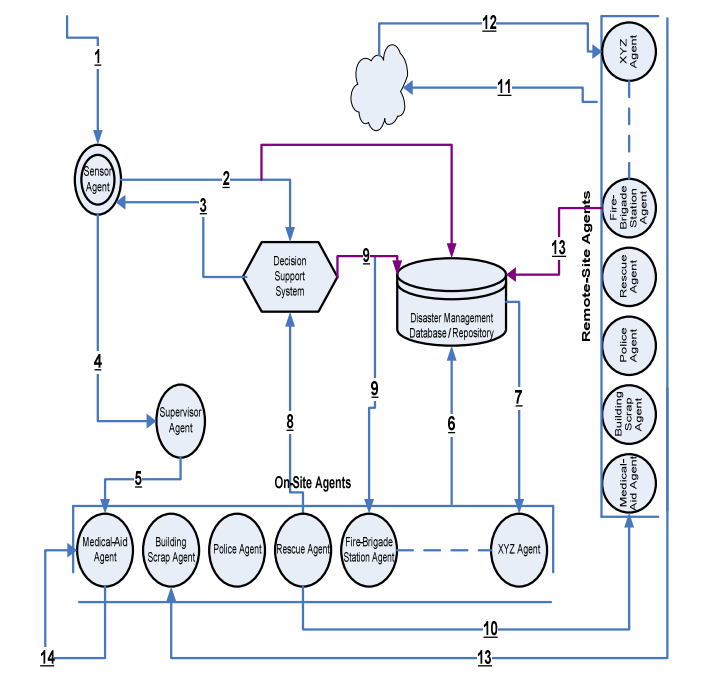
\includegraphics[scale=0.65]{esquem-artigo.png}
    \caption{Arquitetura do \textit{FMSIND}}
\end{figure}

A nossa solução e o estudo descrito anteriormente foram baseados em ferramentas já criadas, nomeadamente:
\begin{itemize}
    \item \textbf{EQ-Rescue} \cite{eqr}, uma ferramenta que simula o aparecimento de tremores de terra e o tratamento deste. Este consiste de 3 módulos: \underline{Disaster World Model}, que é usado para representação do mundo, o \underline{Resource Model}, representante dos recursos existentes e, por fim, o \underline{Emergency Operation Center (EOC)}, módulo responsável pela tomada de decisões;
    \item\textbf{ Knowledge Oriented Sensor Web}\cite{kos}, uma plataforma onde os agentes trabalham cooperativamente para, não só determinar o estado da situação mas também para tomar ações. O sistema consiste em duas partes, uma responsável por avaliar o ambiente e outra por tratar das respostas. Estas ficam ligadas através de uma base de dados e de um sistema de decisão comunicando por específicas mensagens ou através uma plataforma web.
\end{itemize}

\section{Contextualização da Solução}

O mapa da Floresta do simulador é constituído por \textbf{habitações} (locais onde os agentes participativos terrestres não serão capazes de “pisar”), locais de abastecimento de \textbf{água} (rios, mares, lagoas, entre outros) e locais de abastecimento de \textbf{combustível} (bombas de combustível).

No início de cada simulação é gerado um mapa, onde as habitações e os locais de abastecimento de água e de combustível serão distribuídos por posições aleatórias. Posteriormente, o Quartel irá dividir o mapa por \textbf{zonas} (delimitadas por 4 posições, por isso, terão que ser quadradas ou retangulares), sendo que cada uma deverá conter pelo menos um posto de abastecimento de água e de combustível. Em seguida, os agentes serão proporcionalmente distribuídos pelas zonas, ou seja, quanto maior for uma zona, mais agentes participativos estarão encarregues pela mesma. Para além disso, também terá em consideração os diferentes tipos de veículos existentes, de modo a que se encontrem equilibradamente distribuídos por todo o mapa. Essa posição delegada a cada um dos veículos no início da simulação será considerada a sua \textbf{posição ideal}, logo, o bombeiro deverá permanecer nessa posição até ir combater um incêndio e regressar para a mesma assim que o incêndio se extinguir.

Um bombeiro encontrar-se-á sempre num dos seguintes estados: \textbf{em repouso} quando não está encarregue de nenhum incêndio, \textbf{a caminho} para combater um incêndio, \textbf{em ação} quando está a combatê-lo e \textbf{a regressar} quando está a voltar para a sua posição ideal.

Posteriormente, o \textbf{ateador de fogos}, através de uma taxa de probabilidade aleatória e variável, irá gerar um fogo numa posição arbitrária do mapa. Nesta posição não poderão existir habitações, nem postos de abastecimento de água e combustível. Depois de iniciado um fogo, este poderá \textbf{expandir-se} pois estará associado a uma taxa de expansão, que variará de acordo com o tempo de duração do incêndio e com o ambiente circundante (quanto mais húmido, ou seja, com abastecimentos de água, menos probabilidade terá de se expandir, e quando mais seco, isto é, com casas e postos de combustível, maior probabilidade terá).

O Quartel possui uma lista dos fogos ativos que já estão confiados a algum bombeiro, e uma lista de fogos ativos que ainda estão à espera de serem delegados. Assim, a cada momento da simulação, o Quartel consulta a lista de fogos em espera e começa por atribuir bombeiros aos fogos com maior \textbf{gravidade} (que varia de acordo com a distância às habitações, e que estará constantemente a ser reavaliada). O Quartel delegará essa tarefa com base em:

\begin{enumerate}
    \item Zona onde o incêndio se situa: o agente participativo deverá fazer parte dessa zona;
    \item Distância do agente participativo ao incêndio (considerando a velocidade máxima do respetivo tipo de veículo);
    \item Ter água suficiente para combater o determinado incêndio.
\end{enumerate}

Depois de enviado o pedido ao respetivo bombeiro, o mesmo poderá aceitar ou recusar o encargo. Para tomar esta decisão, o próprio bombeiro terá em conta o seu estado interno. Desta forma, se estiver em repouso ou a regressar à sua posição ideal, o bombeiro irá \textbf{aceitar} a tarefa, caso contrário, se estiver já a dirigir-se para outro incêndio ou ocupado a combater algum, irá \textbf{recusar} a tarefa.

Quando um veículo está a dirigir-se ou a regressar de um incêndio e, por mero acaso, aproxima-se demasiado de um outro incêndio, o bombeiro pode \textbf{proativamente} optar por combater esse fogo. Desta forma, este comunicará a sua intenção ao Quartel, que irá avisar o bombeiro que já estava atribuído ao fogo em questão para regressar para a sua posição ideal (caso exista).

Assim que um veículo acabe de combater um incêndio poderá ir \textbf{reabastecer} o seu depósito de água, caso esteja a metade ou menos de metade, abastecendo também o seu depósito de combustível se necessário e, por fim, regressar à sua posição ideal.

No entanto, tal como já referido, quando o Quartel envia um pedido a um agente participativo para combater um incêndio existe a possibilidade da tarefa ser rejeitada. Neste caso, o Quartel pedirá ao segundo veículo que melhor satisfaz as três condições anteriormente mencionadas para combater o fogo. A lista de bombeiros vai sendo percorrida \textbf{ciclicamente} até algum dos bombeiros aceitar a tarefa, e, entretanto, o fogo continuará na lista em espera.

Existe ainda um outro fator que terá que ser tido em conta pelo Quartel no processo de monitorização das catástrofes: a \textbf{taxa de ocupação} da zona. Esta taxa representa o número de fogos a dividir pelo número de agentes participativos presentes numa zona, que, consequentemente, pode ser interpretada como o excesso de incêndios em curso para a quantidade de recursos disponível. Neste caso, se a taxa for demasiado alta (maior que ~150\%), o Quartel realocará temporariamente recursos de zonas com uma menor taxa. Nesta alocação cada bombeiro terá somente como objetivo combater um determinado incêndio, e deverá regressar para a sua posição ideal no final.

\pagebreak
\section{Arquitetura}

\begin{figure}[h!]
    \centering
    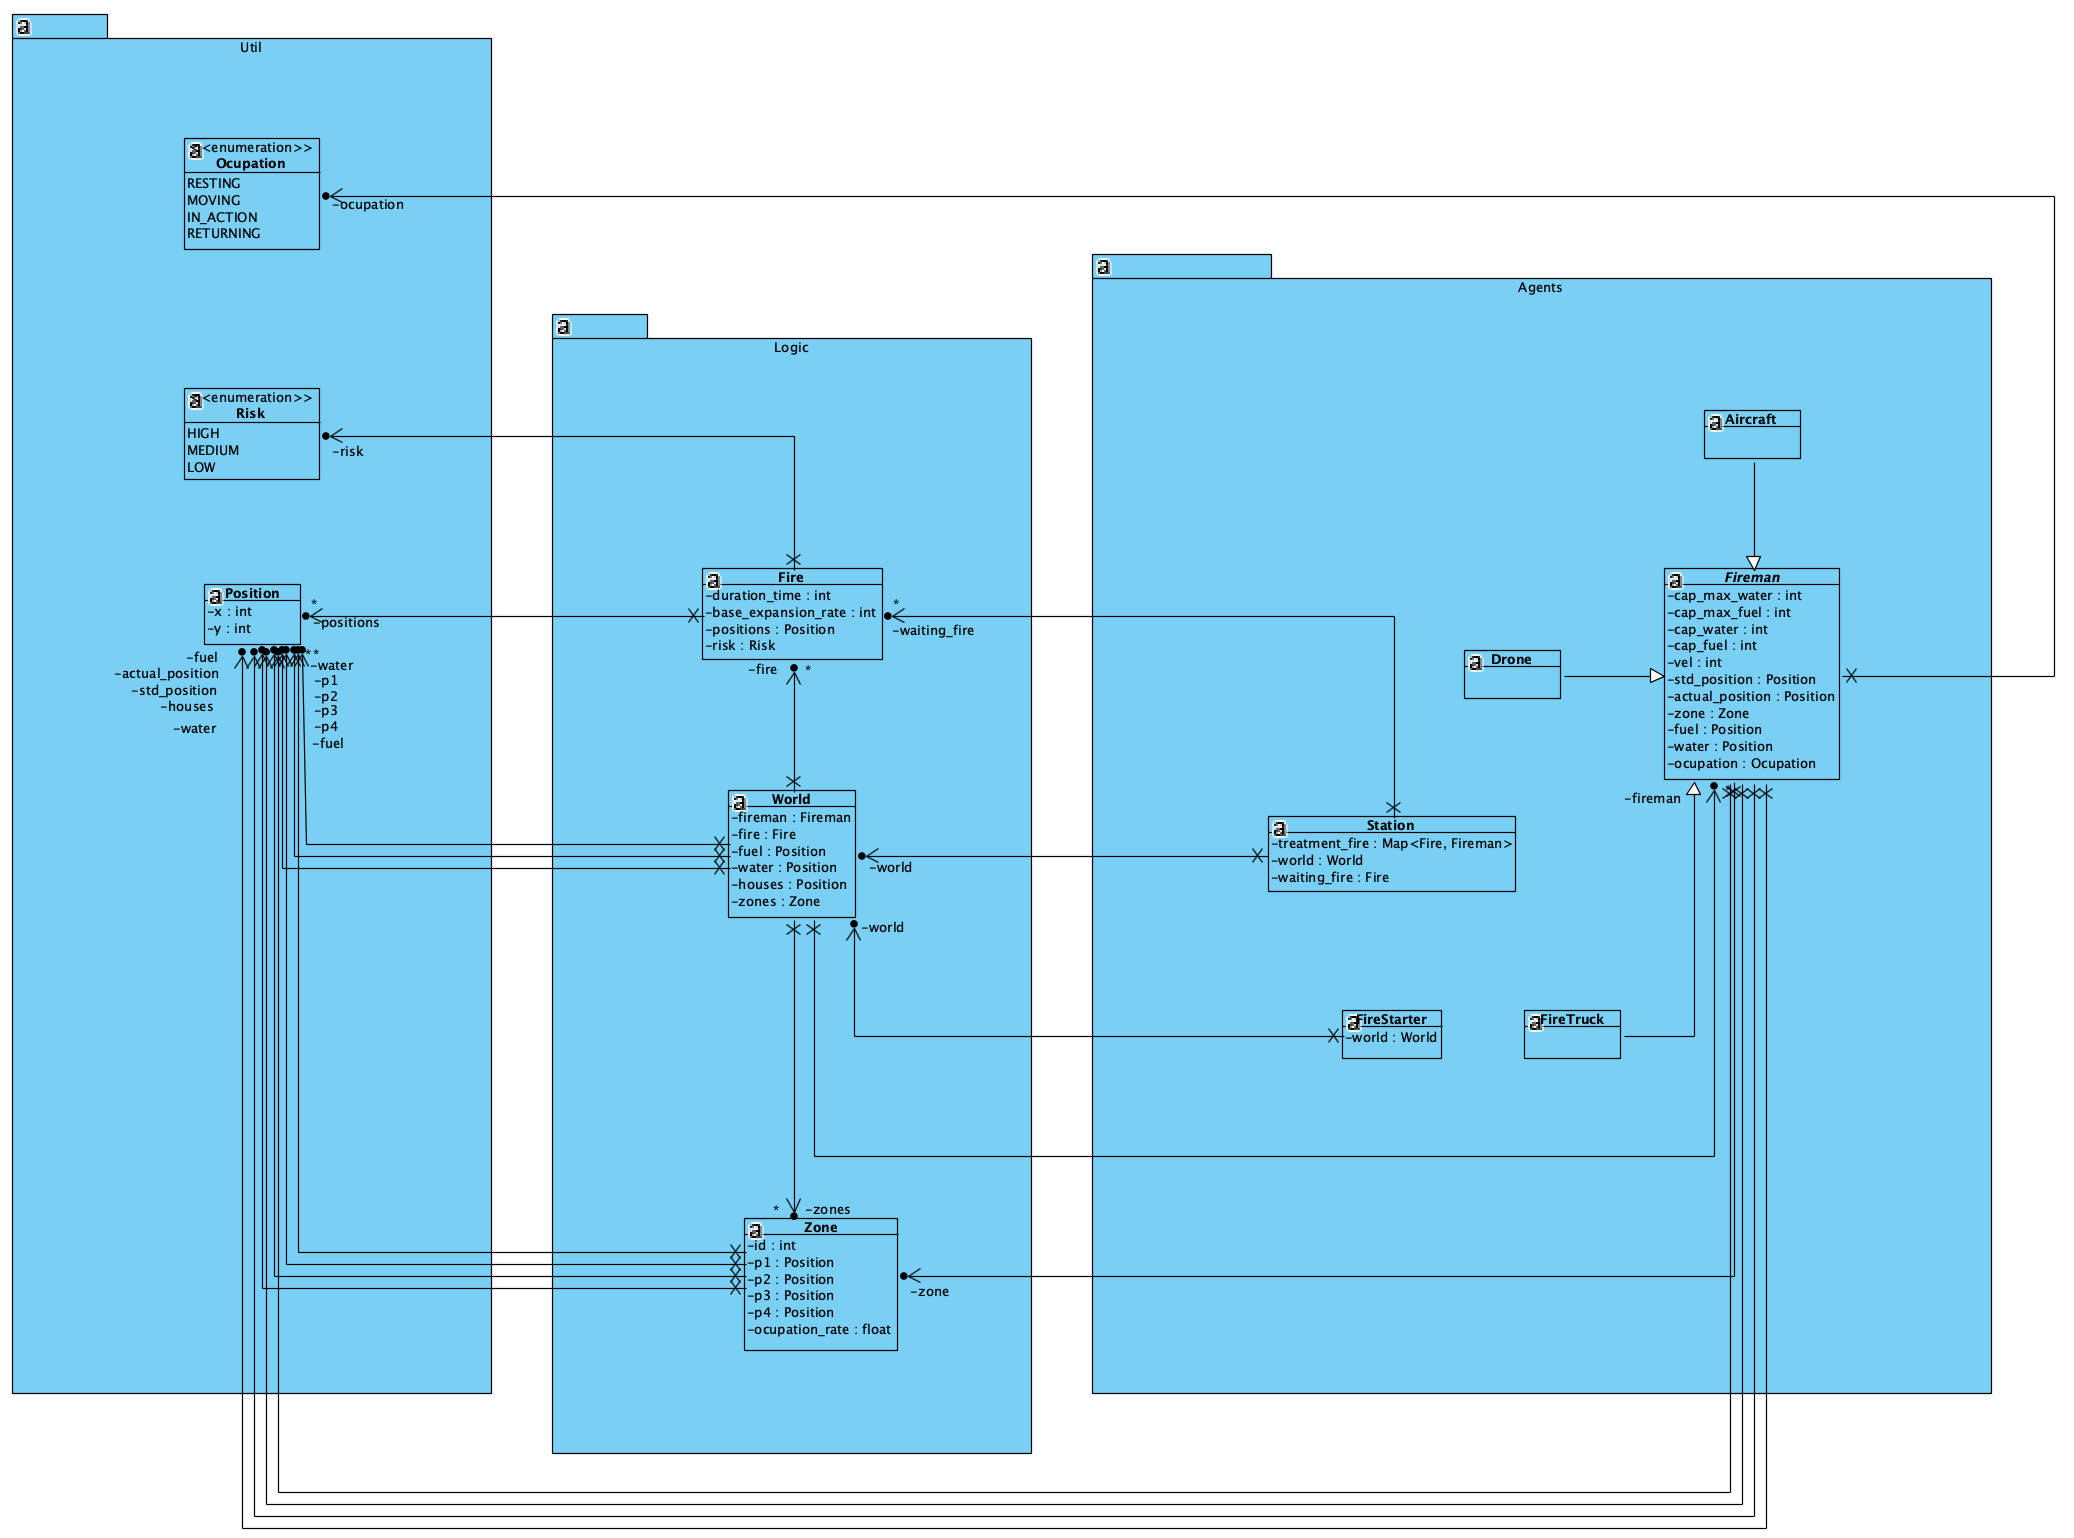
\includegraphics[scale=0.41]{classes.png}
    \caption{Diagrama de Classes.}
    \label{img:classes}
\end{figure}

Para a modelação do nosso sistema multiagente começamos por elaborar um diagrama de classes, presente na Figura~\ref{img:classes}. Em seguida, explicamos as diferentes classes e as respetivas variáveis.

O estado do simulador é da responsabilidade da classe \textbf{\textit{World}}. A disposição do mapa engloba a \textbf{lista dos bombeiros}, a \textbf{lista dos fogos} existentes, a \textbf{lista das posições} dos postos de abastecimento de \textbf{combustível}, \textbf{água} e de \textbf{habitações}. Por fim, possui ainda a \textbf{lista das zonas} existentes no mapa.

A \textit{\textbf{Zone}} tem conhecimento relativo ao seu \textbf{id}, às coordenadas das \textbf{quatro posições} (vértices) que delimitam a respetiva zona e à sua \textbf{taxa de ocupação}, isto é, o número de fogos a dividir pelo número de agentes participativos presentes na zona (se a taxa for demasiado alta, terão que ser enviados temporariamente novos agentes participativos para a zona).

O \textbf{\textit{Fire}} tem uma \textbf{lista de posições} (poderá ser mais do que uma quando o fogo se alastra), uma \textbf{gravidade} (alta, média ou baixa, uma vez que certas posições poderão apresentar habitações nas redondezas), o \textbf{tempo de duração} que o incêndio se apresenta ativo e, por fim, a \textbf{taxa de expansão base} do fogo (relacionada com o ambiente; por exemplo, se tiver próximo de uma zona com água, tem menor probabilidade). A taxa de expansão aplicada será baseada na taxa base e no tempo de duração do fogo.

O Agente Central, \textbf{\textit{Station}}, apresenta conhecimento relativo à \textbf{disposição do mapa}, nomeadamente as posições das habitações, dos locais de abastecimento de combustível e de água, as delimitações das zonas e as informações relativas aos fogos e aos bombeiros. Para além disso, armazena uma \textbf{lista de todos os fogos ativos},o respetivo agente participativo encarregue pelo mesmo e uma \textbf{lista de todos os fogos que estão em espera} (sem nenhum agente encarregue por apagá-lo). 

O Agente Secundário, \textbf{\textit{FireStarter}}, tem acesso ao \textbf{estado do jogo}, o que significa que tem acesso às posições em que não pode atear fogos (habitações, postos de abastecimento de água e combustível e posição dos bombeiros).

O Agente Participativo, \textbf{\textit{Fireman}}, tem como variáveis a sua \textbf{posição ideal} (aquela que lhe é atribuída no início da geração do mapa), a sua \textbf{posição atual}, a \textbf{zona} a que pertence, uma \textbf{lista das posições dos postos de abastecimento de água e combustível} da sua zona, a \textbf{capacidade máxima} e os \textbf{níveis atuais de combustível e água}, a \textbf{velocidade de movimento}, e, por fim, a sua \textbf{ocupação atual}, que poderá ser “Em repouso” (quando está na sua posição ideal e não lhe está atribuído nenhum fogo), “Em deslocação” (quando está a dirigir-se para o fogo), “Em ação” (quando está a apagar o fogo) e “A regressar” (quando está a regressar para a sua posição ideal).

O \textbf{\textit{Fireman}} poderá ser um \textbf{\textit{FireTruck}}, um \textbf{\textit{Drone}} ou um \textbf{\textit{Aircraft}}.

A \textbf{\textit{Position}}, é um par ordenado (X,Y) e corresponde a uma posição do mapa.




\section{Protocolo de Comunicação}
Como seria de esperar, no simulador os agentes irão comunicar entre si de modo a provocarem e resolverem catástrofes naturais.

Para representar estas interações recorremos a diagramas de sequência de sistemas, que refletem as diferentes mensagens que são trocadas entre os agentes, nos diversos momentos da simulação. Estas comunicações serão baseadas nas normas FIPA utilizadas pelo \textit{JADE}, ou seja, utilizaremos \textit{performatives} para indentificar os vários tipos de pedidos envolvidos entre os agentes.

\subsection{Inicia Agente}
\begin{figure}[h!]
    \centering
    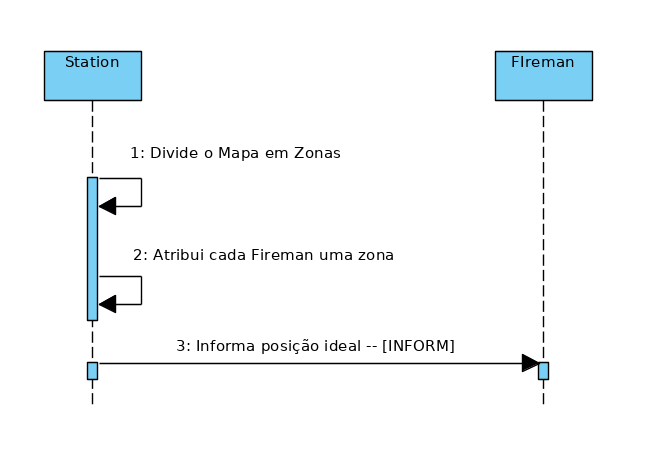
\includegraphics[scale=0.4]{IniciaAgent_v3.png}
    \caption{Diagrama de Sequência correspondente ao início de um bombeiro.}
\end{figure}
Ao iniciar a simulação, o quartel terá de começar por dividir o mapa em várias zonas e atribuir a cada uma destas um número de bombeiros, dos diferentes tipos. Após a seleção, indicará a cada um a sua posição ideal, ou seja, a posição onde deverá permanecer sempre que não estiver em combate.

\pagebreak
\subsection{Agente Informa Estado Atual}
\begin{figure}[!h]
    \centering
    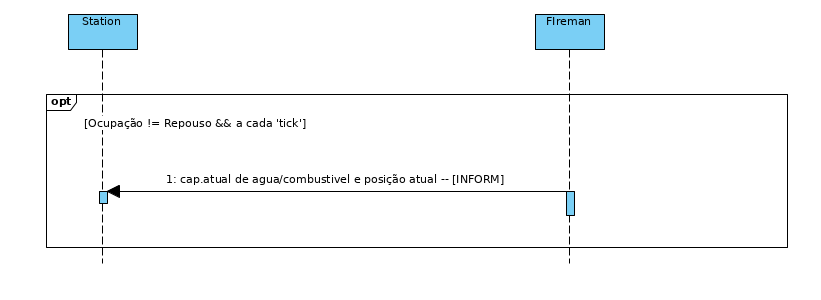
\includegraphics[scale=0.4]{Agente_INforma_Estado_Atual.png}
    \caption{Diagrama de Sequência correspondente à comunicação do bombeiro sobre o seu estado ao quartel.}
\end{figure}
Durante a simulação o quartel terá de saber o estado de cada um dos bombeiros. Por isso, sempre que este estiver ocupado, seja em deslocação ou em combate - se estiver em repouso não terá nada para informar -, e a cada momento da simulação, este enviará uma mensagem a indicar os seus níveis de água e combustível, assim como a sua posição atual.

\subsection{Ateador Inicia Fogo}
\begin{figure}[!h]
    \centering
    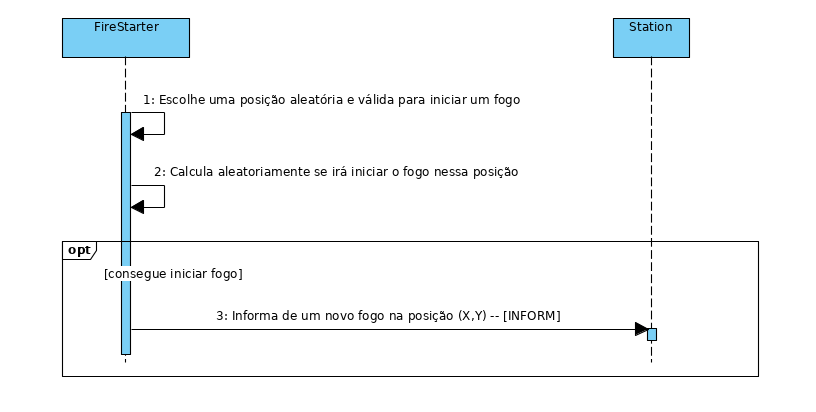
\includegraphics[scale=0.4]{AteadorCriaFogo_V2.png}
    \caption{Diagrama de Sequência correspondente à criação de incêndios.}
\end{figure}
O Ateador de fogos, a cada momento da simulação tenta iniciar um novo fogo. Trata-se somente de uma tentativa, pois apesar de determinar uma posição, válida, para o novo fogo, apenas o concretiza se houver probabilidade (aleatória e variável) para tal.

\pagebreak
\subsection{Deteta Fogo}
\begin{figure}[!h]
    \centering
    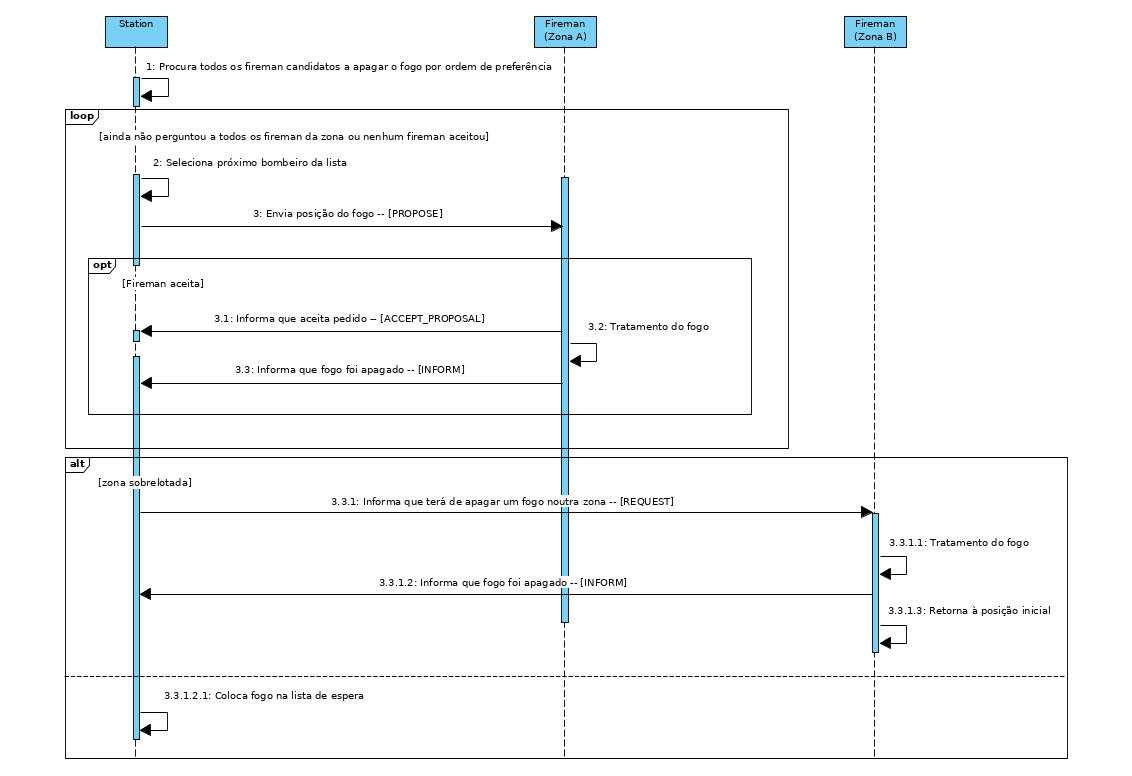
\includegraphics[scale=0.35]{DetetaFogo.png}
    \caption{Diagrama de Sequência correspondente à deteção de um fogo.}
\end{figure}
A cada momento da simulação o Ateador de Fogos irá “tentar” iniciar um novo fogo. Assim que um novo aparecer, o quartel irá detetá-lo e proceder ao seu tratamento. Após determinar o bombeiro mais apropriado dentro da zona onde se encontra o fogo, este irá enviar-lhe uma mensagem a perguntar se aceita apagar o fogo. Se o bombeiro aceitar, notifica o quartel que aceitou, trata o fogo e informa de novo que concluiu a tarefa. Porém, caso não aceite, pergunta ao próximo candidato. Por fim, chegando ao fim da lista e nenhum ter aceite, este verifica se a zona está sobrelotada com fogos e, caso esteja acima de aproximadamente 150\%, aloca um novo agente de uma outra zona não sobrelotada para temporariamente sair da sua zona e apagar o fogo em questão. Se não estiver sobrelotada, simplesmente é colocado em lista de espera para mais tarde ser reavaliado.

\pagebreak
\subsection{Iniciativa de Apagar um Fogo do Agente}
\begin{figure}[!h]
    \centering
    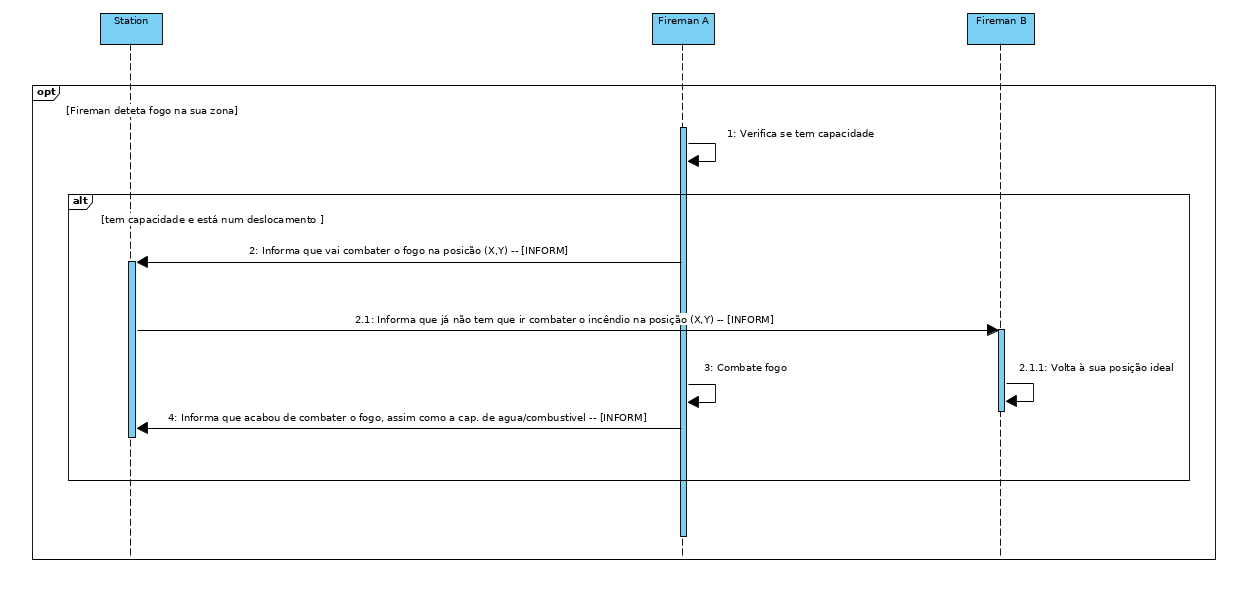
\includegraphics[scale=0.3]{ResolverFogoACaminho_V4.png}
    \caption{Diagrama de Sequência correspondente à resolução de um fogo por iniciativa do bombeiro.}
\end{figure}
Se um bombeiro estiver em regresso de outro fogo ou a caminho de algum, este poderá tomar a iniciativa de apagar um fogo que esteja perto, com algumas condições. Se resolver apagá-lo fá-lo-á depois de notificar o Quartel que irá apagar o respetivo fogo que, por sua vez, informará o bombeiro responsável por este fogo (se houver algum atribuído) que já está a ser tratado e cancelar a ação.

\pagebreak
\section{Processamento Interno dos Agentes}

Os diagramas seguintes são demonstrativos do processamento interno de cada um dos agentes envolvidos no sistema.

\subsection{Agente Incendiário}
Como podemos ver no diagrama este agente só possui dois estados, em repouso e a \textit{incendiar}. O Agente, após se iniciar o programa, fica em repouso até decidir preparar um incêndio. Após esta transição o agente fica no estado a \textit{incendiar}. Quando o programa é terminado, o agente termina consequentemente.
\begin{figure}[!h]
    \centering
    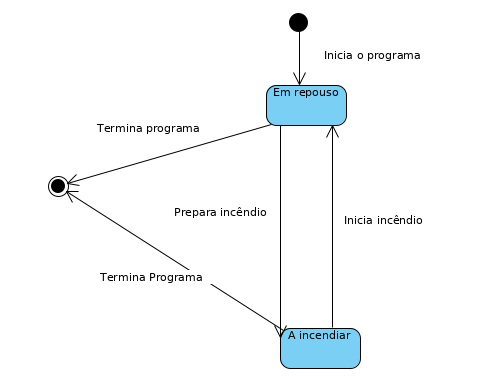
\includegraphics[scale=0.6]{incediario.png}
    \caption{Máquina de estados do Agente Incendiário}
\end{figure}


\subsection{Agente Quartel}
O quartel após iniciar o programa entra num primeiro estado que apenas ocorre dessa vez, calcular posições ideais dos agentes Bombeiro. Após o término desse cálculo os estados bifurcam-se no cálculo de taxas de ocupação das zonas e de risco de incêndio, caso existam, e na procura de incêndios. Assim que é detectado um incêndio transita para o estado de procura do melhor agente para o combate, após encontrar este agente envia-lhe uma mensagem de pedido de ação. Depois disto fica em espera até receber uma resposta. Caso seja positiva transita para a bifurcação inicial, caso seja negativa retorna ao estado de procura de agente. Tal como no agente anterior, caso o programa seja terminado o agente termina com ele.
\begin{figure}[H]
    \centering
    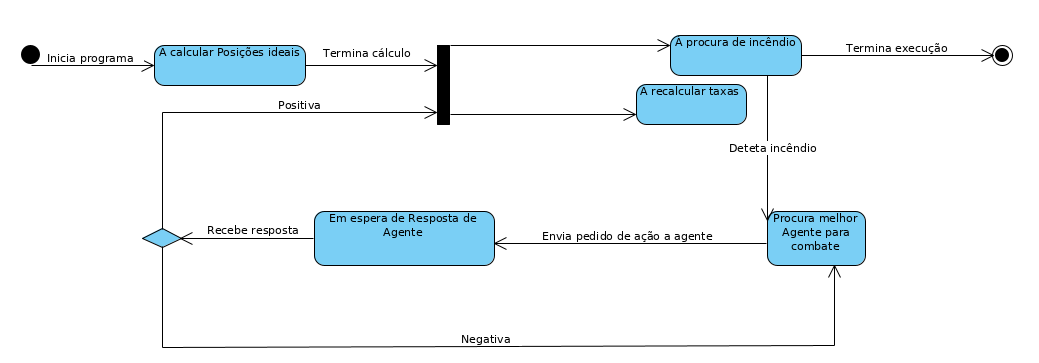
\includegraphics[scale=0.45]{AIQuartel.png}
    \caption{Máquina de estados do Agente Quartel}
\end{figure}

\subsection{Agente Bombeiro}
O agente bombeiro, tal como já foi referido nas secções anteriores, apresenta quatro estados. Após o programa ser inicializado ele recebe a sua posição ótima e começa o deslocamento para essa posição. A partir do momento que chega ao destino fica em espera até receber o pedido de ação, podendo aceitar ou recusar esse pedido. Caso aceite começa a deslocar-se para a posição do incêndio, caso recuse continua em espera. Ao deslocar-se para um incêndio, aquando da chegada passa para o estado em ação. Posteriormente a terminar o combate começa a regressar para a sua posição ideal. No  regresso ou a caminho de um fogo, se detetar um incêndio pode, por iniciativa própria, combater esse fogo.
\begin{figure}[H]
    \centering
    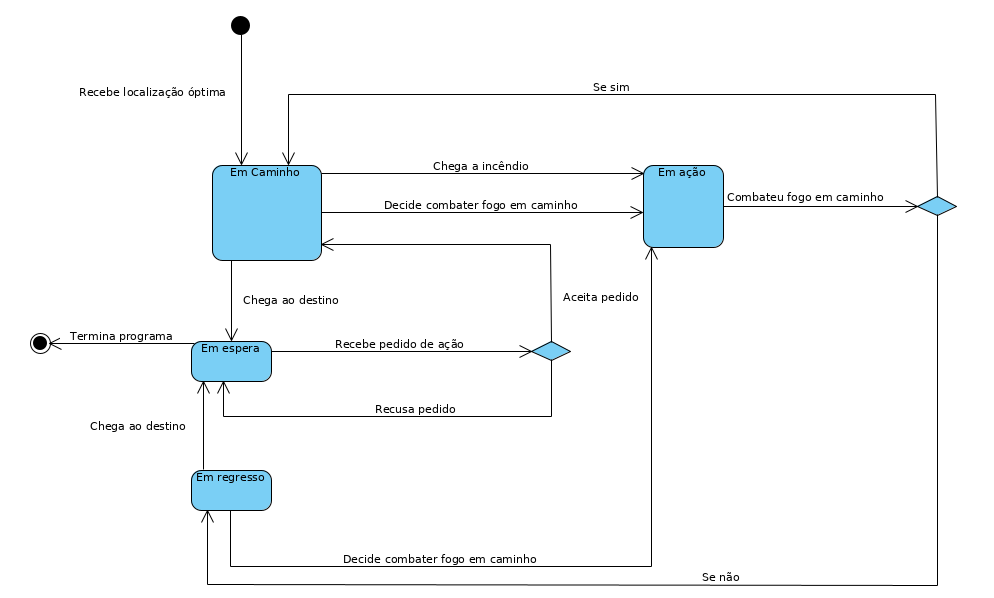
\includegraphics[scale=0.45]{Bombeiro.png}
    \caption{Máquina de estados do Agente Bombeiro}
\end{figure}

\pagebreak
\section{Alterações da Fase 1}

\subsection{Diagrama de Classes Final}
%--- TODO: colocar imagem


\newpage
\section{Conclusão e Trabalho Futuro}
O planeamento do sistema multiagente que visa monitorizar e resolver catástrofes naturais foi, sem dúvida, uma fase determinante para o futuro processo da implementação do simulador.

A tarefa mais complicada ao longo da idealização do sistema foi a tentativa de equilibrar as responsabilidades entre o Quartel (Agente Central) e os Veículos Bombeiros (Agentes Participativos). Desta forma, o objetivo passou por tentar não sobrecarregar o Quartel na seleção do bombeiro mais adequado para resolver o incêndio, visto que existe um vasto leque de variáveis que podem ser consideradas nesta decisão, tais como: a capacidade atual de combustível e de água do bombeiro, a distância do mesmo em relação ao incêndio considerando também as distâncias caso ele tenha que abastecer ao longo caminho (o que faria com que o Quartel tivesse que projetar à partida o trajeto a ser efetuado pelo bombeiro), ou ainda considerar distâncias cruzadas, de forma a que fosse encontrada a solução ótima global.

Como não almejávamos centralizar demasiado a resolução dos incêndios, mas mesmo assim não queríamos prejudicar excessivamente a eficiência da solução, tentamos que o agente participativo interferisse inteligente e ativamente nas decisões. Como tal, optamos por considerar que o Quartel apenas teria em conta a distância em relação ao local do incêndio e se o veículo tem água suficiente para o apagar, desprezando os restantes fatores. O bombeiro tem a possibilidade de recusar o pedido e de proativamente combater um incêndio, caso se cruze com um numa deslocação. Este modelo de deteção e resolução de catástrofes certamente que não conduz o nosso simulador à solução ótima, mas torna os nossos agentes mais autónomos e cooperativos.

Outra das decisões tomadas foi o facto de dividirmos o mapa por zonas, o que faz com que a escolha do melhor veículo seja mais limitada. Porém, consideramos essa limitação benéfica, uma vez que acreditamos que tornará o mapa mais organizado e civilizado.
	
Decidimos também planear desde já alguns fatores extra, como por exemplo o facto dos agentes poderem agir proativamente e do fogo se poder alastrar. Posteriormente, tencionamos estender a lista de pontos complementares, como por exemplo adicionar estradas ao mapa, de forma a tornarmos o nosso simulador o mais verídico possível.

Como trabalho futuro, planeamos focarmo-nos no desenvolvimento do algoritmo que apresentamos na presente fase do projeto e resolver da melhor forma inevitáveis problemas de implementação ou até incongruências de planeamento que surjam. Tentaremos que, para além de conceptualmente conseguirmos representar um simulador o mais real possível, também visualmente seja possível percecionar a participação dos agentes, através de um mapa 2D. Também tencionamos que exista um lugar para a apresentação de resultados estatísticos relativamente à performance dos agentes.

Este trabalho irá, certamente, contribuir para o desenvolvimento das nossas competências técnicas no que diz respeito a ferramentas como \textbf{Java}, \textbf{JADE}, \textbf{JESS}, entre outras \textit{APIs} que serão cruciais para a implementação do simulador, e ainda fortalecerá os nossos conhecimentos relativos a Agentes e a Sistemas Multiagente.\newpage

\begin{thebibliography}{}
\bibitem{fmsind}
Muhammad Aslam, Muhammad Tariq Pervez, Syed Shah Muhammad, Seemal Mushtaq, Ana Maria Martinez Enriquez,
\textit{FMSIND: A Framework of Multi-Agent Systems Interaction during Natural Disaster}
\bibitem{kos}
Xiangyu Si, Jonathan Li, Zhijun Wang, 
\textit{Knowledge-Oriented Sensor Web For Disaster Management: From Sensing To Decision Making}
\bibitem{eqr}
F.Fiedrch, 
\textit{
An HLA-based multiagent system for optimized resource allocation after strong earthquakes
}
\end{thebibliography}{}

\end{document}
